\section{Advanced Continuous Distributions}

In this section we will study three fundamental continuous distributions and a key tool for analyzing them: the moment-generating function.

\subsection{Continuous Uniform Distribution}

The continuous uniform distribution models the case where a random variable takes values in an interval $[a,b]$ with the same probability density at every point.

\begin{definicion}[Continuous Uniform Distribution]
A continuous random variable $X$ has a \emph{continuous uniform distribution} on the interval $[a,b]$, with $a<b$, if its density function is given by
\begin{align}
 \label{eq:2.8.1}
 f(x) =
 \begin{cases}
  \dfrac{1}{b-a} & a \leq x \leq b, \\
  0 & \text{otherwise.}
 \end{cases}
\end{align}
In this case, we write $X \sim U(a,b)$.
\end{definicion}

Its cumulative distribution function is
\begin{align}
 \label{eq:2.8.2}
 F(x) = P(X \leq x) =
 \begin{cases}
  0 & x < a, \\
  \dfrac{x-a}{b-a} & a \leq x \leq b, \\
  1 & x > b.
 \end{cases}
\end{align}

{Properties of the uniform distribution} If $X \sim U(a,b)$, then
\begin{align}
 \mu_X &= \frac{a+b}{2}, \\
 \s_X^2 &= \frac{(b-a)^2}{12}.
\end{align}

\begin{observacion}
The uniform distribution is the foundation of the \emph{simple random sample}: if $X_1,\dots,X_n \sim U(0,1)$ are independent, then $(X_1,\dots,X_n)$ is a uniform sample in the hypercube $[0,1]^n$.
\end{observacion}

\begin{ejemplo}
 \label{exmp:2.8.1}
The waiting time for a bus at a bus stop is uniform on the interval $[0,15]$ minutes. What is the probability that the bus arrives in less than $5$ minutes? What is the expected waiting time?
\end{ejemplo}

\begin{solucion}
Since $X \sim U(0,15)$, the density is $f(x) = \frac{1}{15-0} = \frac{1}{15}$ for $x \in [0,15]$.

The probability that it arrives in less than $5$ minutes is
\begin{align}
 P(X < 5) = \int_0^5 \frac{1}{15}\,dx = \frac{5}{15} = \frac{1}{3}.
\end{align}

The expected waiting time is
\begin{align}
 E(X) = \frac{a+b}{2} = \frac{0+15}{2} = 7.5 \text{ minutes}.
\end{align}
\end{solucion}

\lstinputlisting[language=Python]{../code/distribuciones-continuas-avanzadas/distUniforme.py}

\begin{figure}
 \centering
 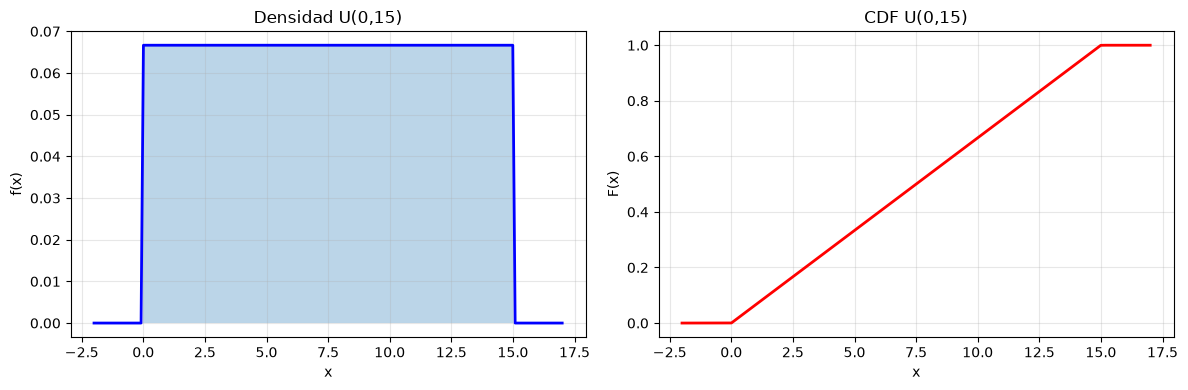
\includegraphics[height=7cm,keepaspectratio=true]{./pe/distUniforme.png}
 % distUniforme.png: 0x0 pixel, 300dpi, 0.00x0.00 cm, bb=
 \caption{Continuous uniform distribution $U(0,15)$: density and CDF.}
 \label{fig:2.8.1}
\end{figure}

\subsection{Normal Distribution}

The normal distribution is the most important continuous distribution in statistics and appears in the \emph{Central Limit Theorem}.

\begin{definicion}[Normal Distribution]
A continuous random variable $X$ has a \emph{normal distribution} with parameters $\mu$ (mean) and $\sigma > 0$ (standard deviation) if its density function is
\begin{align}
 \label{eq:2.8.3}
 f(x) = \frac{1}{\sigma\sqrt{2\pi}}\,\exp\!\left(-\frac{(x-\mu)^2}{2\sigma^2}\right),
 \qquad x \in \mathbb{R}.
\end{align}
We write $X \sim N(\mu, \sigma^2)$.
\end{definicion}

{Properties of the normal distribution} If $X \sim N(\mu,\sigma^2)$, then
\begin{itemize}
 \item The distribution is \emph{symmetric} with respect to $\mu$.
 \item $\mu$ is the mean, median, and mode.
 \item $\sigma^2$ is the variance.
 \item If $Z \sim N(0,1)$ (standard form), then $X = \mu + \sigma Z$.
\end{itemize}

{Standard form} If $X \sim N(\mu, \sigma^2)$, the standardized variable
\begin{align}
 \label{eq:2.8.4}
 Z = \frac{X - \mu}{\sigma}
\end{align}
follows an $N(0,1)$ distribution with density
\begin{align}
 \label{eq:2.8.5}
 \varphi(z) = \frac{1}{\sqrt{2\pi}}\,e^{-z^2/2}, \qquad z \in \mathbb{R}.
\end{align}

{Empirical Rule $68$--$95$--$99.7$} If $X \sim N(\mu,\sigma^2)$, then
\begin{align}
 P(\mu - \sigma \leq X \leq \mu + \sigma) &\approx 0.6827, \\
 P(\mu - 2\sigma \leq X \leq \mu + 2\sigma) &\approx 0.9545, \\
 P(\mu - 3\sigma \leq X \leq \mu + 3\sigma) &\approx 0.9973.
\end{align}

\begin{observacion}
The normal distribution appears in many practical situations: measurement errors, human heights, test scores, etc. Furthermore, by the Central Limit Theorem, the sum (or average) of many independent random variables (under mild conditions) is approximately normal.
\end{observacion}

\begin{ejemplo}
 \label{exmp:2.8.2}
The scores on an exam follow an $N(70, 100)$ distribution (mean $70$, variance $100$, i.e., $\sigma=10$). What percentage of students scored between $60$ and $80$ points?
\end{ejemplo}

\begin{solucion}
We standardize: if $X \sim N(70, 100)$, then
\begin{align}
 P(60 \leq X \leq 80) = P\!\left(\frac{60-70}{10} \leq Z \leq \frac{80-70}{10}\right)
 = P(-1 \leq Z \leq 1).
\end{align}

By the empirical rule, this value is approximately $0.6827 = 68.27\%$. Using tables or software, the exact value is $\Phi(1) - \Phi(-1) = 0.8413 - 0.1587 = 0.6827$.
\end{solucion}

\lstinputlisting[language=Python]{../code/distribuciones-continuas-avanzadas/distNormalContinua.py}

\begin{figure}
 \centering
 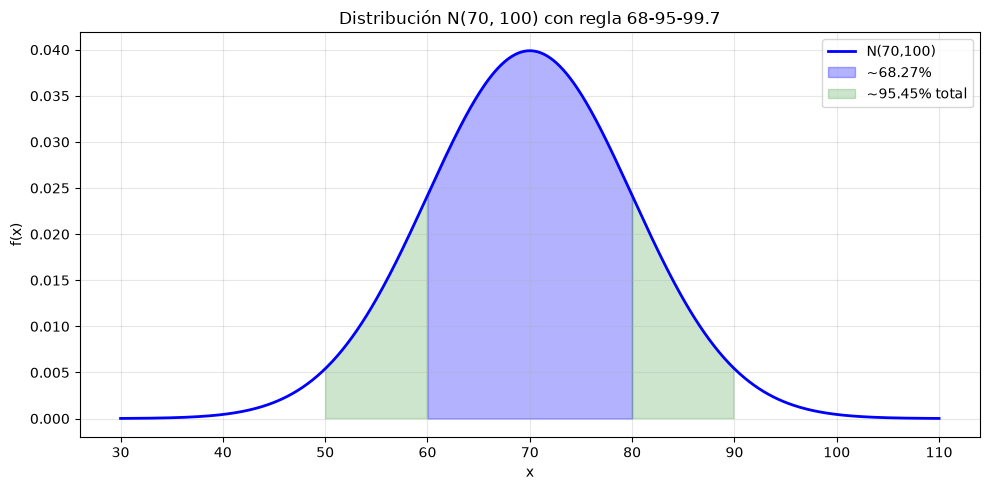
\includegraphics[height=7cm,keepaspectratio=true]{./pe/distNormalContinua.png}
 % distNormalContinua.png: 0x0 pixel, 300dpi, 0.00x0.00 cm, bb=
 \caption{Distribution $N(70,100)$ illustrating the 68--95--99.7 empirical rule.}
 \label{fig:2.8.2}
\end{figure}

\subsection{Gamma-Type Distributions}

The gamma family is a generalization of several important distributions (exponential, chi-square, Erlang) and frequently arises when modeling \emph{waiting times}.

\subsubsection{Gamma Function}

\begin{definicion}[Gamma Function]
The \emph{gamma function} $\Gamma: (0,\infty) \to \mathbb{R}$ is defined as
\begin{align}
 \label{eq:2.8.6}
 \Gamma(\alpha) = \int_0^\infty t^{\alpha-1} e^{-t}\,dt.
\end{align}
\end{definicion}

{Properties of the gamma function}
\begin{itemize}
 \item $\Gamma(1) = 1$.
 \item $\Gamma(\alpha + 1) = \alpha\,\Gamma(\alpha)$ for all $\alpha > 0$.
 \item In particular, for $\alpha \in \mathbb{N}$ we have $\Gamma(n) = (n-1)!$.
 \item $\Gamma(1/2) = \sqrt{\pi}$.
\end{itemize}

\subsubsection{Gamma Distribution}

\begin{definicion}[Gamma Distribution]
A continuous random variable $X$ has a \emph{gamma distribution} with shape parameter $\alpha > 0$ and scale parameter $\beta > 0$ if its density function is
\begin{align}
 \label{eq:2.8.7}
 f(x) =
 \begin{cases}
  \dfrac{1}{\Gamma(\alpha)\,\beta^\alpha}\,x^{\alpha-1}\,e^{-x/\beta},
  & x > 0, \\
  0, & \text{otherwise.}
 \end{cases}
\end{align}
We write $X \sim \text{Gamma}(\alpha, \beta)$.
\end{definicion}

{Properties of the gamma distribution} If $X \sim \text{Gamma}(\alpha, \beta)$, then
\begin{align}
 \mu_X &= \alpha\beta, \\
 \s_X^2 &= \alpha\beta^2.
\end{align}

\subsubsection{Special Case: Exponential Distribution ($\alpha = 1$)}

\begin{definicion}[Exponential Distribution]
A random variable $X$ with distribution $\text{Gamma}(1, \beta)$ is said to have an \emph{exponential distribution} with parameter $\lambda = 1/\beta$. Its density function is
\begin{align}
 \label{eq:2.8.8}
 f(x) =
 \begin{cases}
  \lambda\,e^{-\lambda x}, & x \geq 0, \\
  0, & \text{otherwise.}
 \end{cases}
\end{align}
Its mean and variance are $\mu = 1/\lambda$ and $\sigma^2 = 1/\lambda^2$.
\end{definicion}

\begin{observacion}[Memoryless Property]
The exponential distribution satisfies the \emph{memoryless property}: for $s, t \geq 0$,
\begin{align}
 P(X > s + t \mid X > s) = P(X > t).
\end{align}
It is the only continuous distribution (along with the geometric distribution in the discrete case) possessing this property.
\end{observacion}

\subsubsection{Special Case: Chi-Square Distribution}

The chi-square distribution with $\nu$ degrees of freedom, denoted $\chi^2_\nu$, is a special case of the gamma distribution with parameters $\alpha = \nu/2$ and $\beta = 2$:
\begin{align}
 \label{eq:2.8.9}
 X \sim \chi^2_\nu \iff X \sim \text{Gamma}\!\left(\frac{\nu}{2}, 2\right).
\end{align}
Its density function is
\begin{align}
 f(x) = \frac{1}{2^{\nu/2}\,\Gamma(\nu/2)}\,x^{\nu/2-1}\,e^{-x/2}, \qquad x > 0.
\end{align}

This distribution is studied in detail in Section \ref{sec:3.9} of the inference chapter; its connection with the gamma family allows generalizing several of its properties.

\subsubsection{Sum of Independent Gamma Variables}

\begin{teorema}[Gamma Additive Property]
If $X_1, X_2, \dots, X_n$ are independent random variables with $X_i \sim \text{Gamma}(\alpha_i, \beta)$ (with the same scale $\beta$), then
\begin{align}
 \label{eq:2.8.10}
 Y = X_1 + X_2 + \cdots + X_n \sim \text{Gamma}\!\left(\sum_{i=1}^n \alpha_i,\, \beta\right).
\end{align}
\end{teorema}

\begin{ejemplo}
 \label{exmp:2.8.3}
Calls arrive at a call center according to a Poisson process with rate $\lambda = 3$ calls per minute. What is the distribution of the time until the third call? What is the probability that this time is greater than $1.5$ minutes?
\end{ejemplo}

\begin{solucion}
The time between consecutive calls is exponential with parameter $\lambda = 3$, i.e., $T_i \sim \text{Exp}(3)$ with mean $1/3$ minutes.

By the additive property of the gamma distribution, the time until the third call is
\begin{align}
 T = T_1 + T_2 + T_3 \sim \text{Gamma}(3, 1/3).
\end{align}
Equivalently, $T \sim \text{Erlang}(3, 3)$ with rate parameter $3$.

The probability that $T > 1.5$ is
\begin{align}
 P(T > 1.5) = 1 - F_{\text{Gamma}}(1.5; 3, 1/3) = e^{-3 \cdot 1.5}\left(1 + 3\cdot 1.5 + \frac{(3\cdot 1.5)^2}{2}\right).
\end{align}

Numerically: $3 \cdot 1.5 = 4.5$, so
\begin{align}
 P(T > 1.5) = e^{-4.5}\left(1 + 4.5 + \frac{20.25}{2}\right) = e^{-4.5}(15.625) \approx 0.174.
\end{align}
\end{solucion}

\lstinputlisting[language=Python]{../code/distribuciones-continuas-avanzadas/distGamma.py}

\begin{figure}
 \centering
 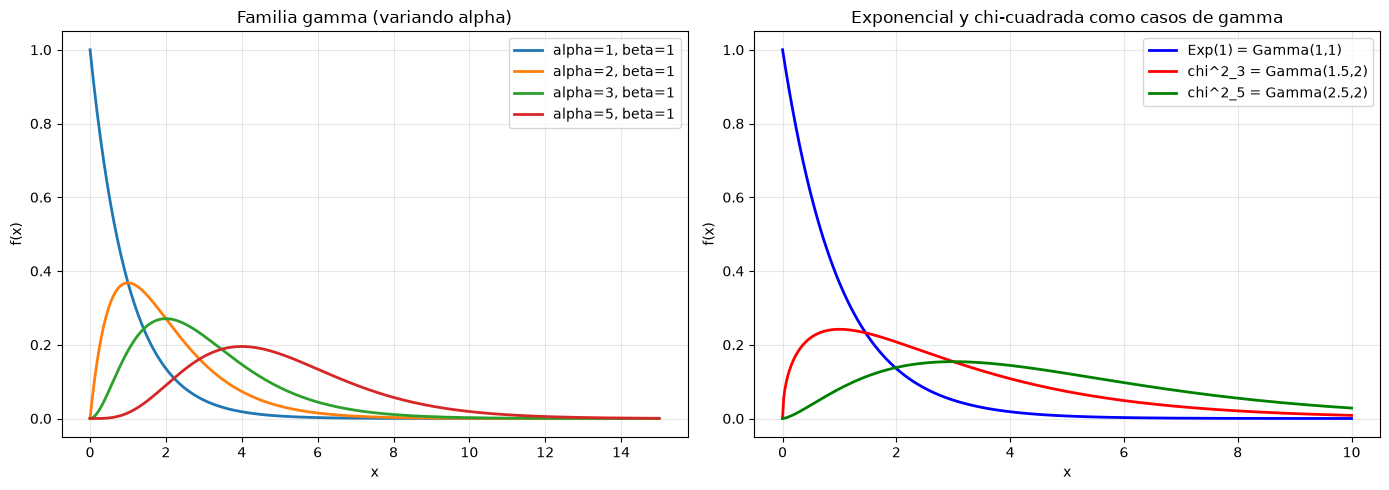
\includegraphics[height=7cm,keepaspectratio=true]{./pe/distGamma.png}
 % distGamma.png: 0x0 pixel, 300dpi, 0.00x0.00 cm, bb=
 \caption{Gamma family and its special cases (exponential and chi-square).}
 \label{fig:2.8.3}
\end{figure}

\subsection{Moment-Generating Function}
\label{sec:mgf}\label{sec:3.4}

The moment-generating function (MGF) is a tool that encodes all the information of a probability distribution into a single function.

\begin{definicion}[Moment-Generating Function]
Let $X$ be a random variable. Its \emph{moment-generating function} (MGF) is
\begin{align}
 \label{eq:2.8.11}
 M_X(t) = E\!\left[e^{tX}\right].
\end{align}
If $X$ is discrete with probability function $f$,
\begin{align}
 M_X(t) = \sum_x e^{tx} f(x).
\end{align}
If $X$ is continuous with density function $f$,
\begin{align}
 M_X(t) = \int_{-\infty}^{\infty} e^{tx} f(x)\,dx.
\end{align}
\end{definicion}

The MGF exists if the integral or sum converges in an open interval around $t=0$.

\subsubsection{Moments from the MGF}

\begin{teorema}[Derivatives and Moments]
If $M_X(t)$ is the MGF of $X$, then for all $n \in \mathbb{N}$,
\begin{align}
 \label{eq:2.8.12}
 E\!\left[X^n\right] = M_X^{(n)}(0) = \left.\frac{d^n M_X(t)}{dt^n}\right|_{t=0}.
\end{align}
\end{teorema}

\begin{proof}
Interchanging differentiation and expectation (under regularity conditions):
\begin{align}
 M_X^{(n)}(t) = \frac{d^n}{dt^n}E[e^{tX}] = E\!\left[\frac{d^n}{dt^n}e^{tX}\right]
 = E\!\left[X^n e^{tX}\right].
\end{align}
Evaluating at $t=0$ yields $M_X^{(n)}(0) = E[X^n]$.
\end{proof}

\subsubsection{Uniqueness and Additive Property}

\begin{teorema}[Uniqueness]
If two random variables have the same MGF on an open interval around $t=0$, then they have the same probability distribution.
\end{teorema}

\begin{teorema}[Additive Property]
If $X$ and $Y$ are independent random variables, then
\begin{align}
 \label{eq:2.8.13}
 M_{X+Y}(t) = M_X(t)\,M_Y(t).
\end{align}
\end{teorema}

\begin{proof}
By independence,
\begin{align}
 M_{X+Y}(t) = E[e^{t(X+Y)}] = E[e^{tX}e^{tY}] = E[e^{tX}]\,E[e^{tY}] = M_X(t)\,M_Y(t).
\end{align}
\end{proof}

\subsubsection{Examples of MGFs}

\begin{ejemplo}
 \label{exmp:2.8.4}
Find the MGF of the Bernoulli distribution with parameter $p$.
\end{ejemplo}

\begin{solucion}
If $X \sim \text{Bernoulli}(p)$, then $P(X=1) = p$ and $P(X=0) = 1-p$.
\begin{align}
 M_X(t) = E[e^{tX}] = e^{0 \cdot t}(1-p) + e^{1 \cdot t}p
 = (1-p) + p\,e^t.
\end{align}

We check the moments:
\begin{align}
 M_X'(t) = p\,e^t &\implies E[X] = M_X'(0) = p. \\
 M_X''(t) = p\,e^t &\implies E[X^2] = M_X''(0) = p. \\
 \text{Var}(X) = E[X^2] - (E[X])^2 &= p - p^2 = p(1-p).
\end{align}
\end{solucion}

\begin{ejemplo}
 \label{exmp:2.8.5}
Find the MGF of the normal distribution $N(\mu, \sigma^2)$.
\end{ejemplo}

\begin{solucion}
Without loss of generality, consider $Z \sim N(0,1)$. Then
\begin{align}
 M_Z(t) &= \int_{-\infty}^{\infty} e^{tz}\,\frac{1}{\sqrt{2\pi}}e^{-z^2/2}\,dz \\
 &= \int_{-\infty}^{\infty} \frac{1}{\sqrt{2\pi}}\,\exp\!\left(tz - \frac{z^2}{2}\right)dz.
\end{align}

We complete the square: $tz - z^2/2 = -\frac{1}{2}(z - t)^2 + \frac{t^2}{2}$. Therefore,
\begin{align}
 M_Z(t) = e^{t^2/2}\int_{-\infty}^{\infty} \frac{1}{\sqrt{2\pi}}e^{-(z-t)^2/2}\,dz = e^{t^2/2}.
\end{align}
(the integral equals $1$ because it is the integral of the $N(t, 1)$ density function).

For $X \sim N(\mu,\sigma^2)$ we write $X = \mu + \sigma Z$, hence
\begin{align}
 \label{eq:2.8.14}
 M_X(t) = E[e^{tX}] = e^{t\mu}E[e^{t\sigma Z}] = e^{t\mu}\,e^{(\sigma t)^2/2}
 = \exp\!\left(\mu t + \frac{\sigma^2 t^2}{2}\right).
\end{align}
\end{solucion}

\begin{ejemplo}
 \label{exmp:2.8.6}
Find the MGF of the exponential distribution with parameter $\lambda$.
\end{ejemplo}

\begin{solucion}
If $X \sim \text{Exp}(\lambda)$, then
\begin{align}
 M_X(t) = \int_0^\infty e^{tx}\,\lambda e^{-\lambda x}\,dx
 = \lambda\int_0^\infty e^{-(\lambda - t)x}\,dx = \frac{\lambda}{\lambda - t},
\end{align}
for $t < \lambda$. Therefore,
\begin{align}
 \label{eq:2.8.15}
 M_X(t) = \frac{\lambda}{\lambda - t} = \left(1 - \frac{t}{\lambda}\right)^{-1},
 \qquad t < \lambda.
\end{align}

The moments are obtained by differentiation:
\begin{align}
 E[X^n] = \frac{n!}{\lambda^n}.
\end{align}
In particular, $E[X] = 1/\lambda$ and $\text{Var}(X) = 1/\lambda^2$.
\end{solucion}

\lstinputlisting[language=Python]{../code/distribuciones-continuas-avanzadas/fgmDistribuciones.py}

\begin{figure}
 \centering
 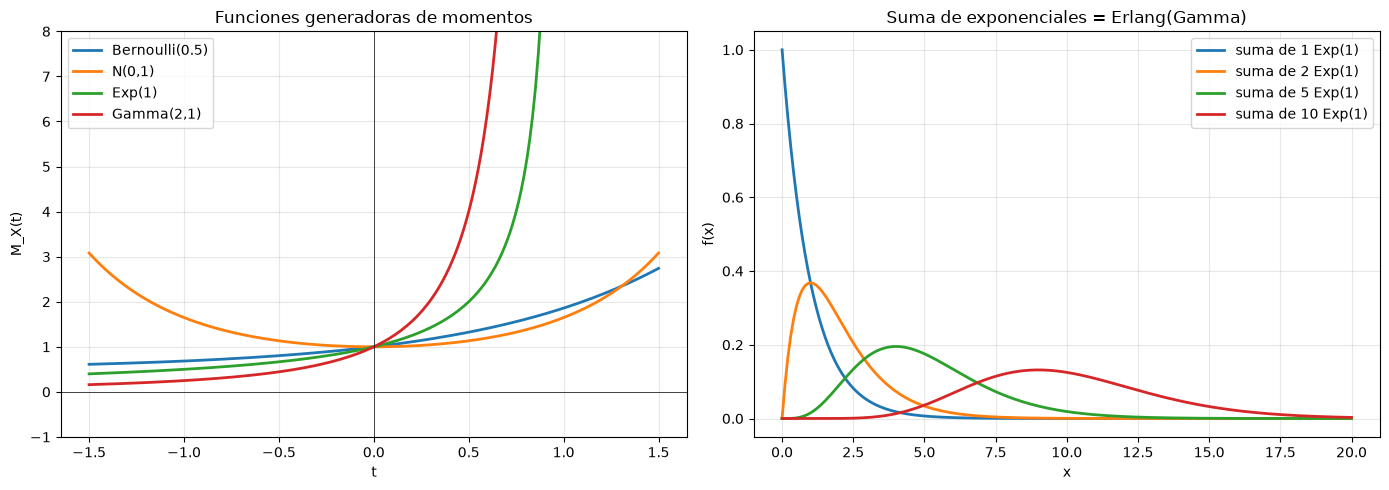
\includegraphics[height=7cm,keepaspectratio=true]{./pe/fgmDistribuciones.png}
 % fgmDistribuciones.png: 0x0 pixel, 300dpi, 0.00x0.00 cm, bb=
 \caption{Moment-generating functions and sum of independent gamma variables.}
 \label{fig:2.8.4}
\end{figure}

{Summary Table of MGFs}
\begin{center}
\begin{tabular}{|l|l|}
\hline
\textbf{Distribution} & \textbf{MGF $M_X(t)$} \\
\hline
Bernoulli$(p)$ & $(1-p) + p\,e^t$ \\
Binomial$(n,p)$ & $(1 - p + p\,e^t)^n$ \\
Poisson$(\lambda)$ & $\exp(\lambda(e^t - 1))$ \\
Geometric$(p)$ & $\dfrac{p\,e^t}{1 - (1-p)e^t}$ \\
Exponential$(\lambda)$ & $\dfrac{\lambda}{\lambda - t}$ \\
Normal$(\mu, \sigma^2)$ & $\exp\!\left(\mu t + \dfrac{\sigma^2 t^2}{2}\right)$ \\
Gamma$(\alpha, \beta)$ & $(1 - \beta t)^{-\alpha}$ \\
Chi-square$_\nu$ & $(1 - 2t)^{-\nu/2}$ \\
\hline
\end{tabular}
\end{center}

\begin{observacion}
The additive property for independent random variables is easily applied: if $X_1, \dots, X_n$ are i.i.d. Bernoulli$(p)$, then $\sum X_i \sim \text{Binomial}(n,p)$ and
\begin{align}
 M_{\sum X_i}(t) = \prod_{i=1}^n M_{X_i}(t) = (1 - p + p\,e^t)^n,
\end{align}
which coincides with the MGF of the binomial distribution.
\end{observacion}
